\chapter{Benchmarking Neuromorphic Vision-Paper 2}
\label{cha:bench}
\section{Introduction}
Despite the promising research on SNN-based vision recognition, there is no commonly-used database in the format of spike stimuli.
In the studies listed above, all of the vision data used are in one of the following formats:
(1) raw grey-scale images data;
(2) pixel-intensity-driven rate-based Poisson spike trains;
(3) unpublished spike-based videos recorded from DVS silicon retinas.
However, in the field of conventional non-spiking computer vision, there are a number of datasets playing important roles at different times and with various objectives.
The MNIST~\cite{lecun1998gradient} dataset is a subset of the NIST hand-written digits dataset; due to its straightforward target of classifying real-world images, the plain format of the binary data and simple patterns, MNIST has been one of the most popular datasets in computer vision for over 20 years.
ImageNet~\cite{deng2009imagenet} was put forward to provide researchers with a large-scale image database that currently contains 14,197,122 images;
this dataset is a well-recognised benchmark test for the deep learning community, and many attempts have been made to improve the performance of machine learning algorithms on this dataset, as was done, for example, by \cite{krizhevsky2012imagenet}.
As a good example of a database catching up with state-of-the-art technologies, Microsoft COCO aims to solve three problems - objects categorisation, context understanding and spatial labelling - in scene understanding by providing large-scale datasets (300,000+ images).
Similar examples can be found in video datasets.
Two early benchmarks, the KTH ~\cite{schuldt2004recognizing} and Weizmann~\cite{blank2005actions} datasets, have been used extensively in the past decade. 
These videos were produced with scripted behaviours in a controlled environment (``in the lab'').
The YouTube Action Dataset~\cite{liu2009recognizing} targets recognising realistic actions from videos ``in the wild'';
here the main challenge is in the massive variations due to the moving camera, background clutter, viewing angles, variable illumination and so on.

In consequence, a new set of spike-based vision datasets is now needed to quantitatively measure progress within this rapidly advancing field and to provide resources to support fair competition between researchers.
Apart from using spikes instead of the frame-based data used in conventional computer vision, new concerns arise when evaluating neuromorphic vision in addition to recognition accuracy.
Therefore a set of common metrics for performance evaluation in spike-based vision is required to assess algorithms and models, including evaluating
trade-offs between simulation time, accuracy and power consumption.
%Benchmarking neuromorphic hardware with various network models will reveal the advantages and disadvantages of different platforms.
Running various SNN benchmarks demonstrates the capability of a hardware platform to support model-specific configurations such as network size, topology, neural and synaptic models, learning algorithms and so on.
In this paper we propose a large dataset of spike-based visual stimuli and a complementary evaluation methodology.
Just as research in this field is an expanding and evolving activity, the dataset will be adapted and extended to fit new requirements presented by advances in the field.
\section{Methods}
\label{sec:method}
\subsection{Guiding Principles}
The NE database we propose here is a developing and evolving dataset consisting of various spike-based representations of images and videos.
The spikes are either generated from spike encoding methods which convert images or frames of videos into spike trains, or recorded from DVS silicon retinas.
The spike trains are in the format of Address-Event Representation~(AER)~\cite{mahowald1992vlsi} data, which are suitable for both event-driven computer simulations and neuromorphic systems.
AER was originally proposed as a time-multiplexed spike communication protocol where each time a neuron produces a spike an event is generated that codes the spiking neuron's address on a fast time-multiplexed digital bus.
The recorded AER data consists of a list of events, each one containing the time stamp of a spike and the address of the neuron which generated the spike.
With the NE dataset we hope:
\begin{itemize}
	\item \textit{to promote meaningful comparisons of algorithms in the field of spiking neural computation.}
	The NE dataset provides a unified format of AER data to meet the demands of spike-based visual stimuli.
	It also encourages researchers to publish and contribute their data to build up the NE dataset.
	\item \textit{to allow comparison with conventional image recognition methods.}
	We expect the dataset to support this comparison using spiking versions of existing vision datasets.
	Thus, conversion methods are required to transform datasets of images and frame-based videos into spike stimuli.
	With the growing understanding of biological vision, new methodologies and algorithms that can convert these conventional datasets into spikes in more biologically-accurate ways are welcome.
	\item \textit{to provide an assessment of the state of the art in spike-based visual recognition on neuromorphic hardware.}
	In order to reveal the advantages of neuromorphic engineering, we need not only a spike-based dataset but also an appropriate evaluation methodology.
	The evaluation methodology will be constantly improving along with the evolution of the dataset.
	\item \textit{to help researchers identify future directions and advance the field.}
	The development of the dataset and its evaluation methodology will introduce new challenges for the neuromorphic engineering community.
	However, these must represent an appropriate degree of challenge: a too-easily-solved problem turns into a tuning competition, while a problem that is too difficult will not yield meaningful assessment.
	So suitable problems should continuously be added to promote future research.  
\end{itemize}


\subsection{The Dataset: NE15-MNIST}
\label{sec:data}
%Experiment setup/ collection method/ properties of each class/ etc.
The first proposed dataset in the benchmarking system is NE15-MNIST (Neuromorphic Engineering 2015 on MNIST).
NE15-MNIST is the spiking version of an original non-spiking dataset which was downloaded from the MNIST Database of Handwritten Digits~\cite{lecun1998gradient}  website\footnote{http://yann.lecun.com/exdb/mnist/}. The converted set consists of four subsets which were generated for different purposes:
\begin{itemize}
	\item \textit{Poissonian},
	which encodes each pixel as a Poisson spike train and is intended for benchmarking existing rate-based SNN models.
	\item \textit{FoCal~(Filter Overlap Correction ALgorithm)},
	to promote the study of spatio-temporal algorithms applied to recognition tasks using small numbers of input spikes.
	\item \textit{DVS recorded flashing input},
	to encourage research into fast recognition methods to mimic the rapid and accurate ``core recognition'' in the primate ventral visual pathway~\cite{dicarlo2012does}.
	\item \textit{DVS recorded moving input},
	to trigger the study of algorithms targeting continuous input from real-world sensors for implementation, for example, on mobile neuromorphic robots.
\end{itemize}
The dataset can be found in the GitHub repository at: https://github.com/NEvision/NE15.
\subsection{Data Description}
\begin{figure}[bt!]
	\centering
%	\subfloat[A snapshot of jAER playing the DVS recorded spikes.]{
%		\label{Fig:jaer}
%		\includegraphics[width=0.22\textwidth]{dvs-128}
%	}
%	\subfloat[A snapshot of jAER playing Poissonian spike trains.]{
%		\label{Fig:poisson}
%		\includegraphics[width=0.22\textwidth]{zero-28-2}
%	}\\
%	\subfloat[The raster plot of the Poissonian spike trains.]{
%		\label{Fig:raster}
%		\includegraphics[width=0.48\textwidth]{zero}
%	}
	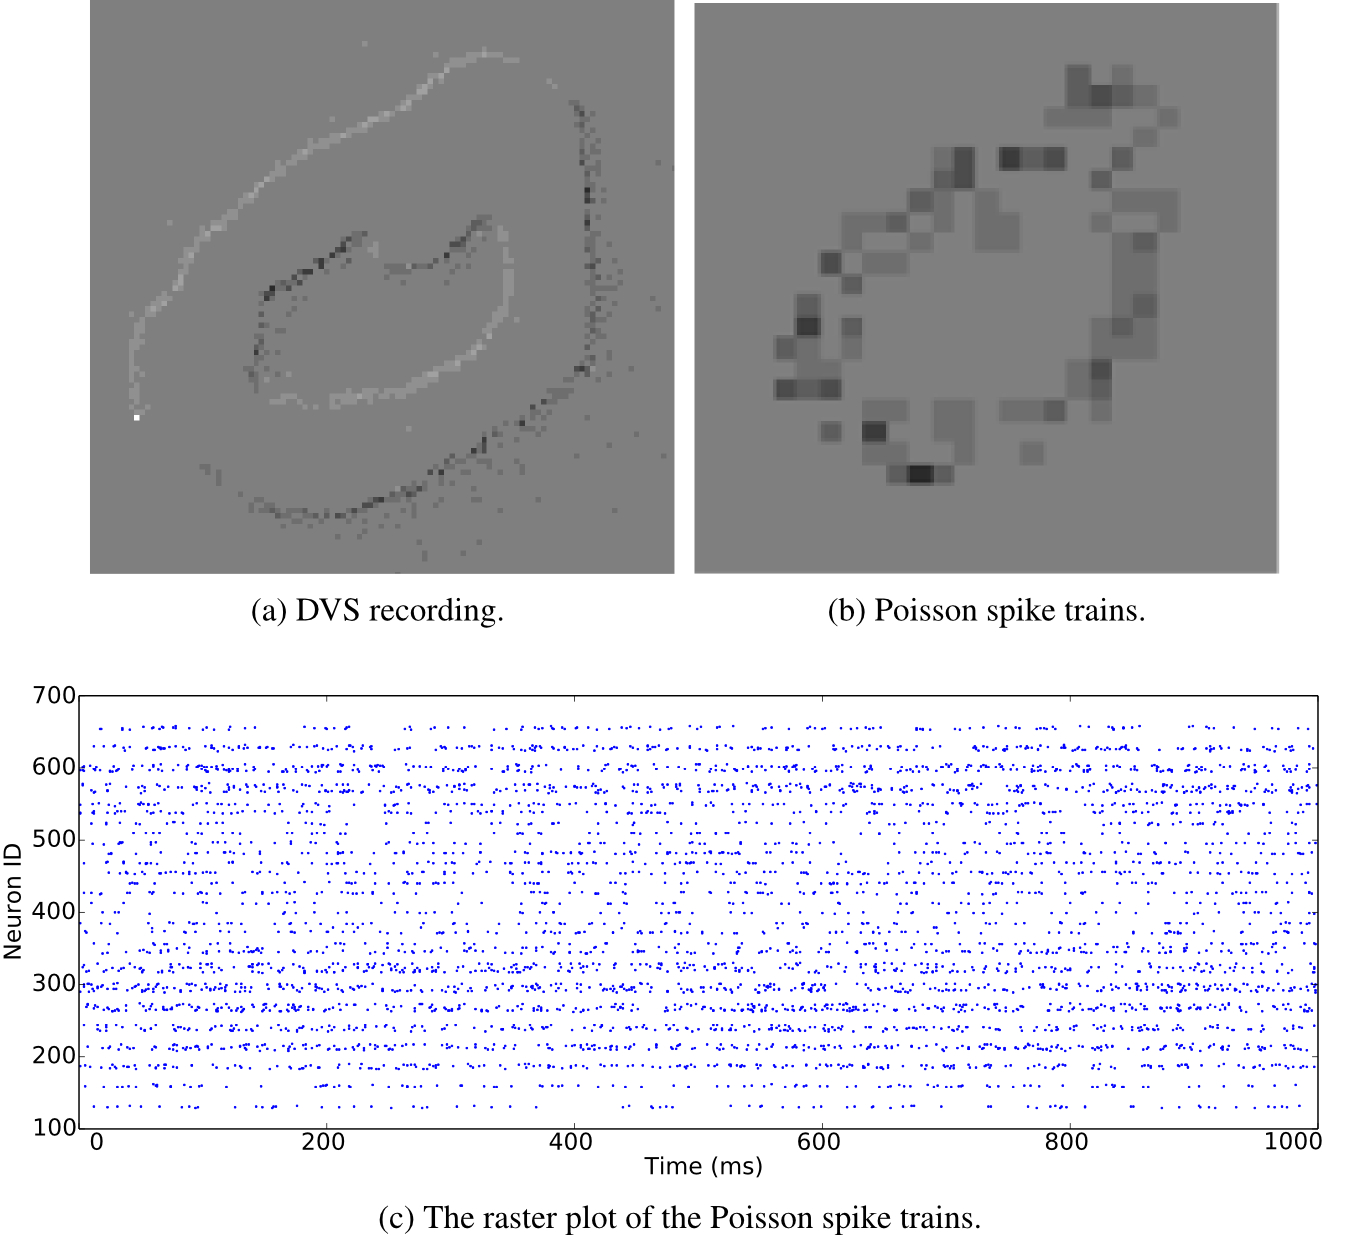
\includegraphics[width=0.75\textwidth]{pics_bench/fig1}
	\caption{
		Snapshots of the jAER software displaying spike-encoded videos.
		The same image of digit ``0'' is transformed into spikes by (a) DVS recording and (b) Poisson generation.
		(c) A raster plot of the Poisson spike trains.}
	\label{fig:zero}
\end{figure}
Two file formats are supported in the dataset: the jAER format~\cite{delbruck2008frame} (.dat or .aedat), and binary files in NumPy~\cite{numpyPython} (.npy) format.
%The AER interface has been widely used in neuromorphic systems, especially for vision sensors.
%The spikes are encoded as time events with corresponding addresses to convey information.
The spikes in jAER format, whether recorded from a DVS retina or artificially generated, can be displayed by the jAER software.
Figure~\ref{fig:zero}(a) is a snapshot of the software displaying a .aedat file which was recorded from a DVS retina~\cite{serrano2013128}.
The resolution of the DVS recorded data is 128$\times$128.
The second spike-based format used is a list of spike source arrays in PyNN~\cite{davison2008pynn}, a description language for building spiking neuronal network models.
Python code is provided for converting from either file format to the other.
The duration of the artificially-generated data can be configured using the Python code provided, while the recorded data varies in duration: 1~s for the flashing input, and 3.2 to 3.4~s for the moving input.



%\subsubsection{Data Description}	
\subsubsection{Poissonian}
\label{sec:poissonian}
The timing of spikes in the cortex is highly irregular~\cite{squire1998findings}.
%In the cortex, the timing of spikes is highly irregular~\cite{squire1998findings}.
An interpretation is that the inter-spike interval reflects a random process driven by the instantaneous firing rate.
If the generation of each spike is assumed to be independent of all other spikes, the spike train is seen as a Poisson process.
The spike rate can be estimated by averaging the pooled responses of the neurons.

As stated above, rate coding is generally used in presenting images as spike trains.
The spike rate of each neuron accords with the intensity of the corresponding pixel.
Instead of providing exact spike arrays, we share the Python code for generating the spikes.
Each recognition system may require different spike rates and durations.
The generated Poisson spike trains can be in both jAER and PyNN spike source array formats.
Thus, it is easy to visualise the digits and also to couple the spike trains into spiking neural networks.
Because different simulators generate random Poisson spike trains with different mechanisms, languages and codes, using the same dataset enables performance evaluation on different simulators without the confusion created by differences in input.
The same digit displayed in Figure~\ref{fig:zero}(a) can be converted into Poisson spike trains, see Figure~\ref{fig:zero}(b).
A raster plot of the Poisson spike trains is shown in Figure~\ref{fig:zero}(c).



\subsubsection{Rank-Order-Encoding}
A different way of encoding spikes is to use a rank-order code; this means
keeping just the order in which the spikes fired and disregarding their exact timing. Rank-ordered spike trains have been used in vision tasks under a biological plausibility constraint, making them a viable way of encoding images for neural applications~\cite{van2001rate,sen2009evaluating,masmoudi2010novel}.

Rank-ordered encoding can be performed using an algorithm known as the
{FoCal algorithm~\cite{sen2009evaluating}}.
This algorithm models the foveal pit region, the highest resolution area of the retina, with four ganglion cell layers each with a different scale of centre-surround receptive field~\cite{kolb2003retina}. In order to simulate these layers two steps are required: the first consists of four discrete 2D convolutions; the second removes redundant information produced in the first step. During the first step, the centre-surround behaviour of the ganglion cells is modelled using Difference of Gaussians~(DoG) kernel for convolution. 
\begin{equation}
\label{eq-dog}
DoG_w(x,y) = \pm\frac{1}{2\pi\sigma_{w,c}^2}e^{\frac{-(x^2 + y^2)}{2\sigma_{w,c}^2}}
\mp\frac{1}{2\pi\sigma_{w,s}^2}e^{\frac{-(x^2 + y^2)}{2\sigma_{w,s}^2}}
\end{equation}
where $\sigma_{w,c}$ and $\sigma_{w,s}$ are the standard deviation of the 
centre and surround components of the DoG at layer $w$. The signs 
will be ($-$,$+$) if the ganglion cell has an OFF-centre behaviour and 
($+$,$-$) if it has an ON-centre one. Table~\ref{tab-kernel-specs} 
describes the parameters used to compute the convolution kernels at each 
scale $w$.

\begin{table}[htb]
	\caption{Simulation parameters for FoCal ganglion cells}
	\begin{center}
		
		
%		\bgroup
%		\def\arraystretch{0.1}
		
		\begin{tabular}{c c c c c c}
			\begin{mycellS}{0.8cm}\centering Layer \end{mycellS}& 
			\begin{mycellS}{1.1cm}\centering Centre type\end{mycellS}& 
			\begin{mycellS}{1.1cm}\centering Matrix width \end{mycellS}&  
			\begin{mycellS}{1.6cm}\centering Centre std. dev. ($\sigma_c$)\end{mycellS} & 
			\begin{mycellS}{1.6cm}\centering Surround std. dev. ($\sigma_s$)\end{mycellS} & 
			\begin{mycellS}{1.3cm}\centering Sampling resolution (cols,rows)\end{mycellS} \\
			\hline
			\begin{mycell}{0.8cm} 1  \end{mycell} &
			\begin{mycell}{1.1cm} \textsc{OFF} \end{mycell}& 
			\begin{mycell}{1.1cm} 3 \end{mycell}& 
			\begin{mycell}{1.6cm}$0.8$ \end{mycell}& 
      \begin{mycell}{1.6cm}$6.7 \times \sigma_c$ \end{mycell}&  
      \begin{mycell}{1.6cm}1, 1 \end{mycell}\\
			\begin{mycell}{0.8cm} 2 \end{mycell} & 
			\begin{mycell}{1.1cm} \textsc{ON} \end{mycell} & 
			\begin{mycell}{1.1cm} 11 \end{mycell}& 
			\begin{mycell}{1.6cm}$1.04$ \end{mycell}& 
      \begin{mycell}{1.6cm}$6.7 \times \sigma_c$ \end{mycell}& 
      \begin{mycell}{1.6cm}1, 1 \end{mycell}\\
			\begin{mycell}{0.8cm} 3 \end{mycell} &
			\begin{mycell}{1.1cm} \textsc{OFF}\end{mycell} & 
			\begin{mycell}{1.1cm} 61 \end{mycell}& 
			\begin{mycell}{1.6cm}$8$ \end{mycell}& 
      \begin{mycell}{1.6cm}$4.8 \times \sigma_c$ \end{mycell}& 
      \begin{mycell}{1.6cm}5, 3\end{mycell} \\
			\begin{mycell}{0.8cm} 4  \end{mycell} & 
			\begin{mycell}{1.1cm} \textsc{ON} \end{mycell} & 
			\begin{mycell}{1.1cm} 243 \end{mycell} &
			\begin{mycell}{1.6cm}$10.4$\end{mycell} & 
      \begin{mycell}{1.6cm}$4.8 \times \sigma_c$\end{mycell} & 
      \begin{mycell}{1.6cm}5, 3 \end{mycell}
		\end{tabular}
%		\egroup
	\end{center}
	\label{tab-kernel-specs}
\end{table}

Every pixel value in the convolved image (Figure~\ref{fig-convolution-results}) 
is inversely proportional to the spike emission time relative to the presentation of the image (i.e. the higher the pixel value, the sooner the spike will fire.)

\begin{figure}[hbt]
	\centering
%	\subfloat[Original image]{
%		\label{sfig-rank-ordered-original}
%		\includegraphics[width=0.15\textwidth]{original_21-0}
%	}
%	\subfloat[Layer 1 (\textsc{off}-centre)]{
%		\label{sfig-rank-ordered-midget-off}
%		\includegraphics[width=0.15\textwidth]{filtered-21-0-layer-0}
%	}
%	\subfloat[Layer 2 (\textsc{on}-centre)]{
%		\label{sfig-rank-ordered-midget-on}
%		\includegraphics[width=0.15\textwidth]{filtered-21-0-layer-1}
%	}\\
%	\subfloat[Layer 3 (\textsc{off}-centre)]{
%		\label{pic-lena-P-OFF}
%		\includegraphics[width=0.15\textwidth]{filtered-21-0-layer-2}
%	}
%	\subfloat[Layer 4 (\textsc{on}-centre)]{
%		\label{pic-lena-P-ON}
%		\includegraphics[width=0.15\textwidth]{filtered-21-0-layer-3}
%	}
	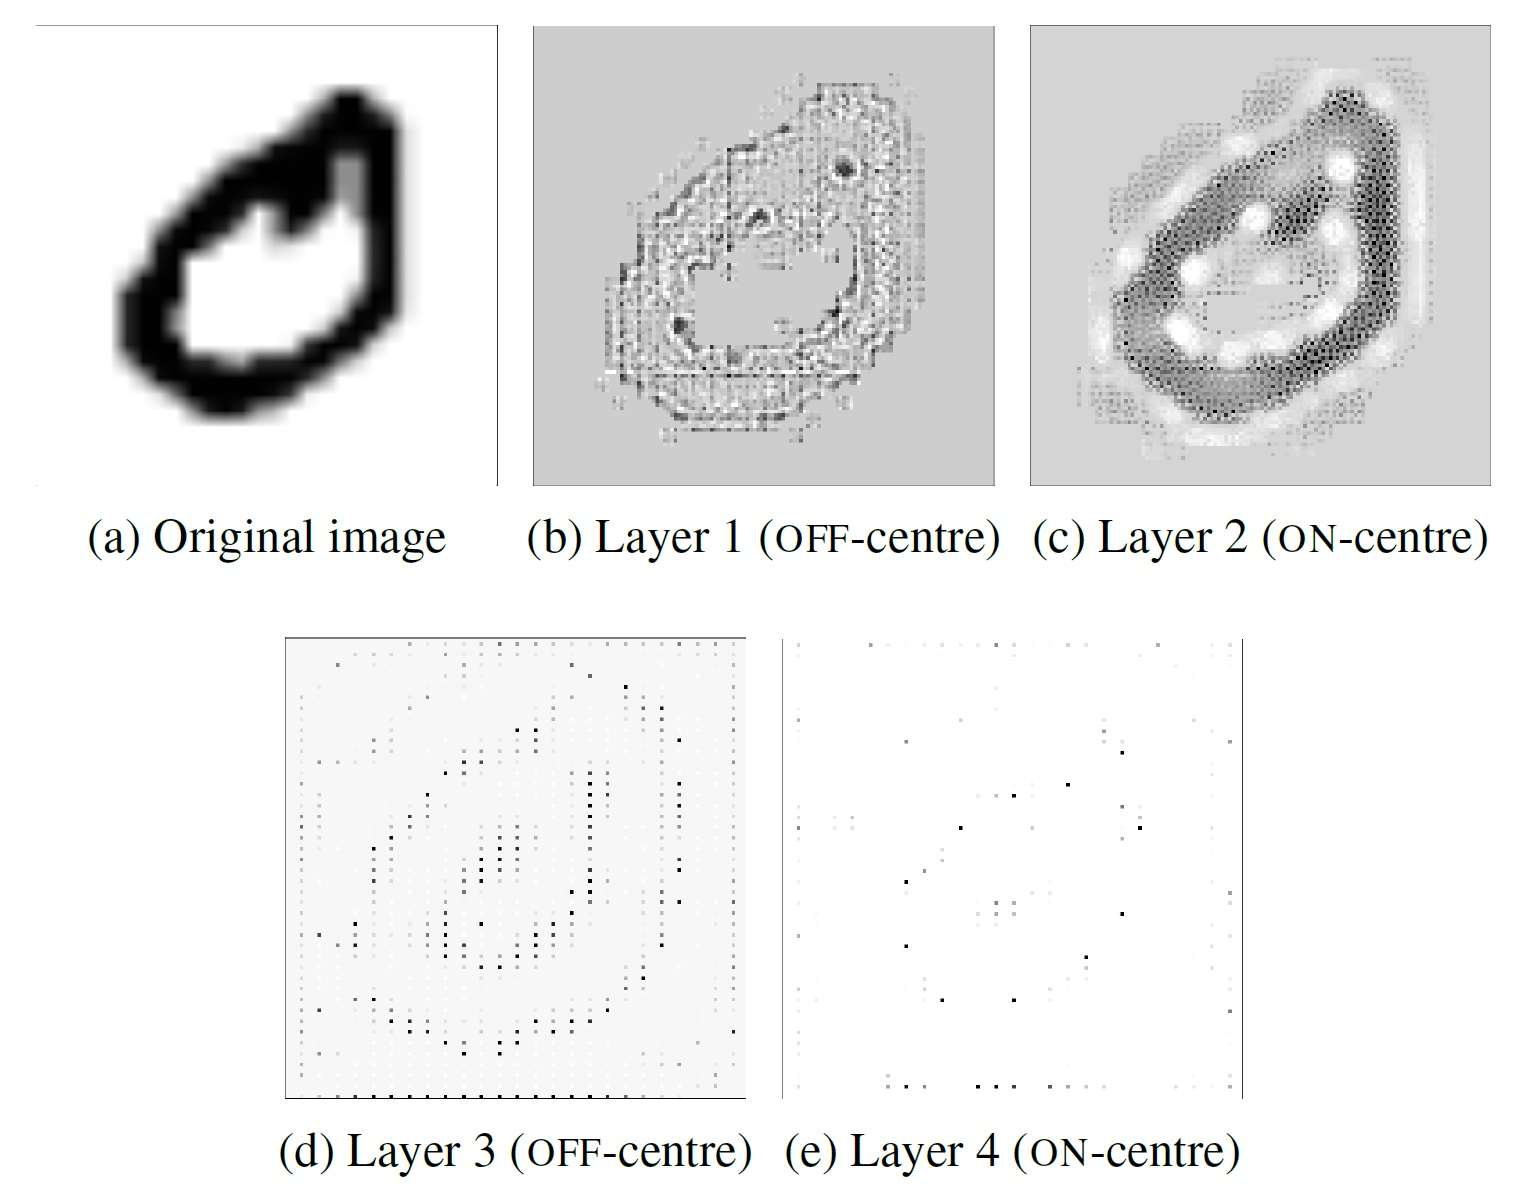
\includegraphics[width=0.6\textwidth]{pics_bench/fig2}
	\caption{Results of convolving the image spikes with the simulated ganglion cell layers using the FoCal algorithm before correcting for filter overlap. (a) The original image. (b-e) the result of convolving the image with the layer 1 (smallest) OFF-centre to layer 4 (largest) ON-centre kernels respectively.}
	\label{fig-convolution-results}
\end{figure}

Since DoGs are used as the means to encode the image, and they do not form an orthogonal set of basis functions, the algorithm also performs a redundancy correction step.
It does so by adjusting the convolved images' pixel values according to the correlation between convolution kernels (Alg.~\ref{code-focal-corr}).

\begin{algorithm}[h]
	\caption{FoCal, redundancy correction}
	\label{code-focal-corr}
	\begin{algorithmic}
		\Procedure{Correction}{coeffs $C$, correlations $Q$}
		\State $N \leftarrow \emptyset$ \Comment{Corrected coefficients}
		\Repeat
		\State $m \leftarrow max(C)$\Comment{Obtain maximum from $C$}
		\State $M \leftarrow M \cup m$\Comment{Add maximum to $M$}
		\State $C \leftarrow C \setminus m$\Comment{Remove maximum from $C$}
		\ForAll{$ c \in C$} \Comment{Adjust all remaining $c$}
		\If{$Q(m, c) \neq 0$} \Comment{Adjust only spatially near coefficients}
		\State $c \leftarrow c - m \times Q(m, c)$
		\EndIf
		\EndFor
		\Until{$C = \emptyset$}
		\State \textbf{return} $M$
		\EndProcedure
	\end{algorithmic}
\end{algorithm}


After the correction step, the most important information can be recovered using only the first 30\% of the spikes~\cite{sen2009evaluating}. These most significant spikes are shown in Figure~\ref{fig-raster-plot-30pc}, which shows the spikes firing at 1~ms intervals. Neurons in Layer 1 emit spikes faster and in larger quantities than any other layer, making it the most important layer. Layers 2 and 3 have few spikes due to the large convolution kernels used to simulate the ganglion cells. One of the main advantages of ROC is that a neuron will only spike once, as can be seen particularly clearly in these two layers. Layers 0 and 1 encode fine detail which can be used to identify what is in the image, while layers 2 and 3 result in blob-like features that should prove useful to location problems.

\begin{figure}[hbt]
	\centering
	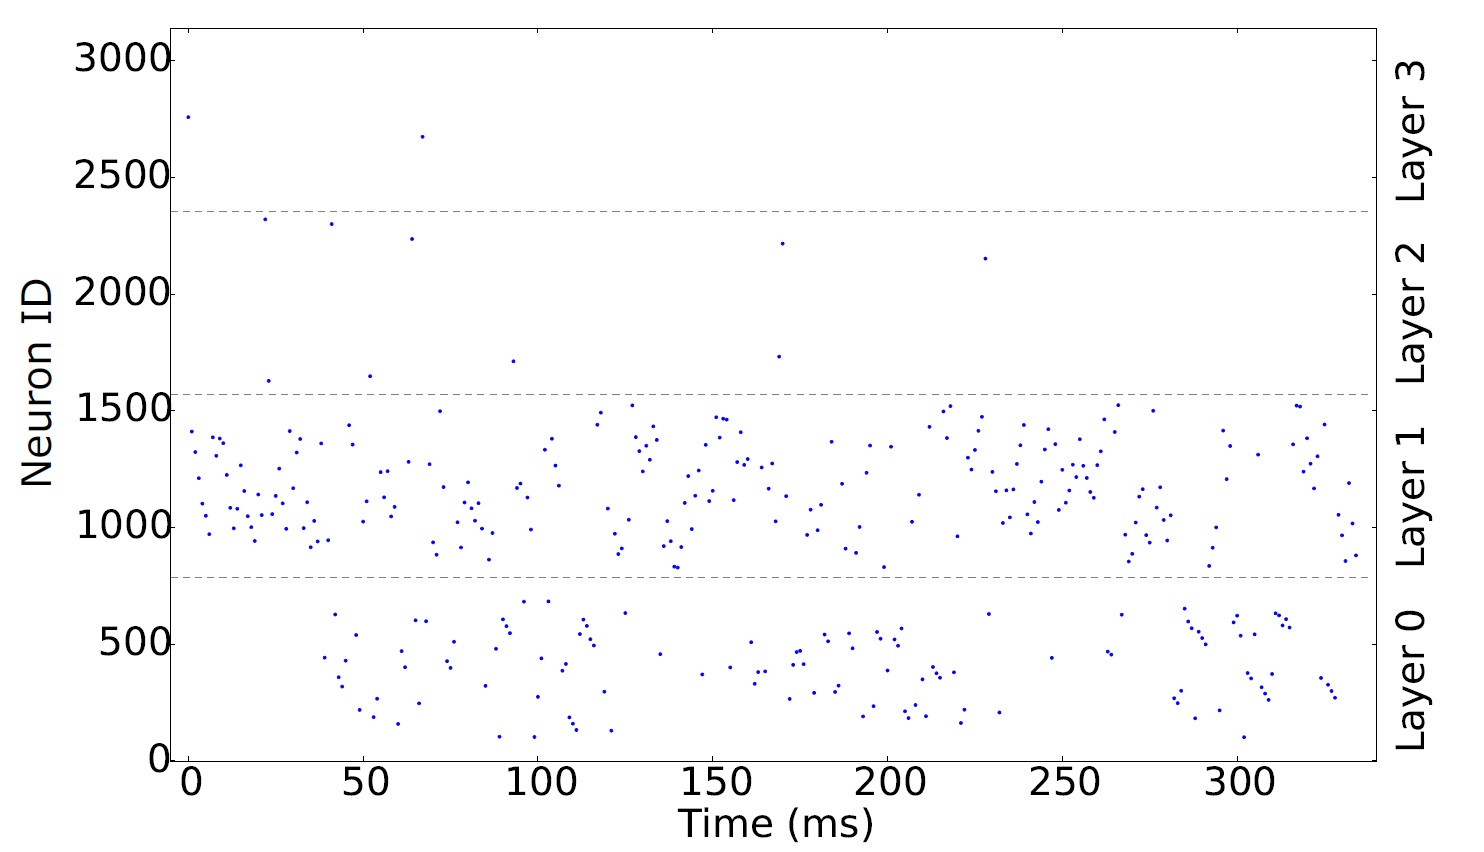
\includegraphics[width=0.48\textwidth]{pics_bench/fig3}
	\caption{Raster plot showing the first 30\% of the rank-order encoded spikes produced using FoCal at 1~ms intervals.}
	\label{fig-raster-plot-30pc}
\end{figure}

Figure~\ref{fig-reconstruction-results} shows the reconstruction results for the two stages of the algorithm. In Figure~\ref{fig-reconstruction-results}(b) the reconstruction was applied after the convolution but without the FoCal correction; a blurry image is the result of redundancy in the spike representation. A better reconstruction can be obtained after Algorithm~\ref{code-focal-corr} has been applied; the result is shown in Figure~\ref{fig-reconstruction-results}(c).


\begin{figure}[hbt]
	\centering
%	\subfloat[Original image]{
%		\label{sfig-rank-ordered-original-1}
%		\includegraphics[width=0.15\textwidth]{original_21-0}
%	}
%	\subfloat[No correction]{
%		\label{pic-lena-reconstructed-raw}
%		\includegraphics[width=0.15\textwidth]{reconstructed_21-0_raw}
%	}
%	\subfloat[FoCal]{
%		\label{pic-lena-reconstructed-focal}
%		\includegraphics[width=0.15\textwidth]{reconstructed_21-0_100pc}
%	}
	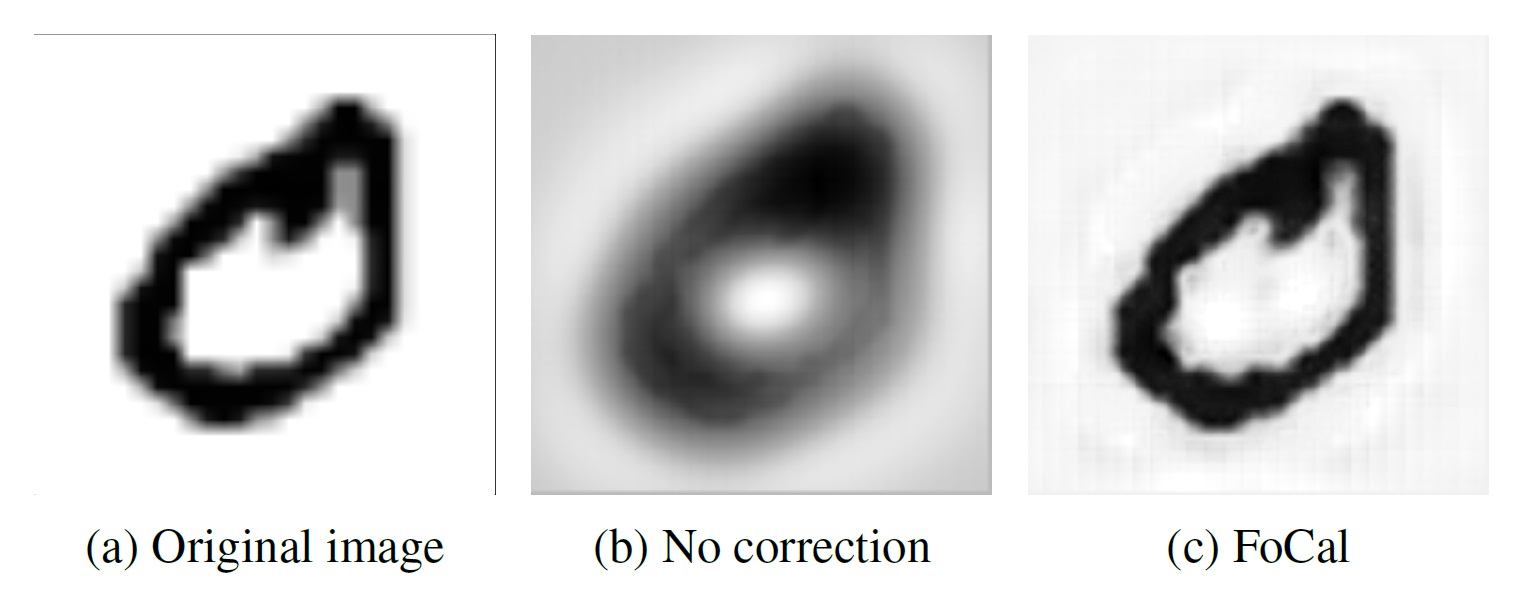
\includegraphics[width=0.6\textwidth]{pics_bench/fig4}
	\caption{Reconstruction result comparison. (a) The original image. (b) Reconstruction without overlap correction. (c) Reconstruction with overlap correction.}
	\label{fig-reconstruction-results}
\end{figure}

The source Python scripts to transform images to ROC spike trains, and to convert the results into AER and PyNN spike source arrays, can be found in the dataset website.

\subsubsection{DVS Sensor Output with Flashing Input}
\label{subsec_flash}
The purpose of including the subset with DVS-recorded flashing digits is to promote research into rapid and accurate ``core recognition'', thus to encourage applying non-rate-based algorithms, for example ROC, to short DVS output spike trains.

Each digit was shown alternating with a blank image and each display lasted one second.
The digits were displayed on an LCD monitor in front of the DVS retina~\cite{serrano2013128} and were placed in the centre of the visual field of the camera.
Since there are two spike polarities - `ON' indicating an increase in the intensity while `OFF' indicates a decrease - there are `ON' and `OFF' flashing recordings respectively per digit.
In Figure~\ref{fig:flash}, the burstiness of the spikes is illustrated where most of the spikes occur in a 30~ms time slot. 
In total, this subset of the database contains 2$\times$$60,000$ recordings for training and 2$\times$$10,000$ for testing.

\begin{figure}[hb!]
	\centering
%	\subfloat[Spikes recorded in the order of neuron ID during 1s of time.]{
%		\label{fig:flash_all}
%		\includegraphics[width=0.48\textwidth]{flash_full}
%	}
%	\\
%	\subfloat[Spikes plotted in the sequence of appearing time during 1s of time. Bursty spikes apeer in slots less than 30~ms. ]{
%		\label{fig:flash_a}
%		\includegraphics[width=0.48\textwidth]{flash_full_order}
%	}
	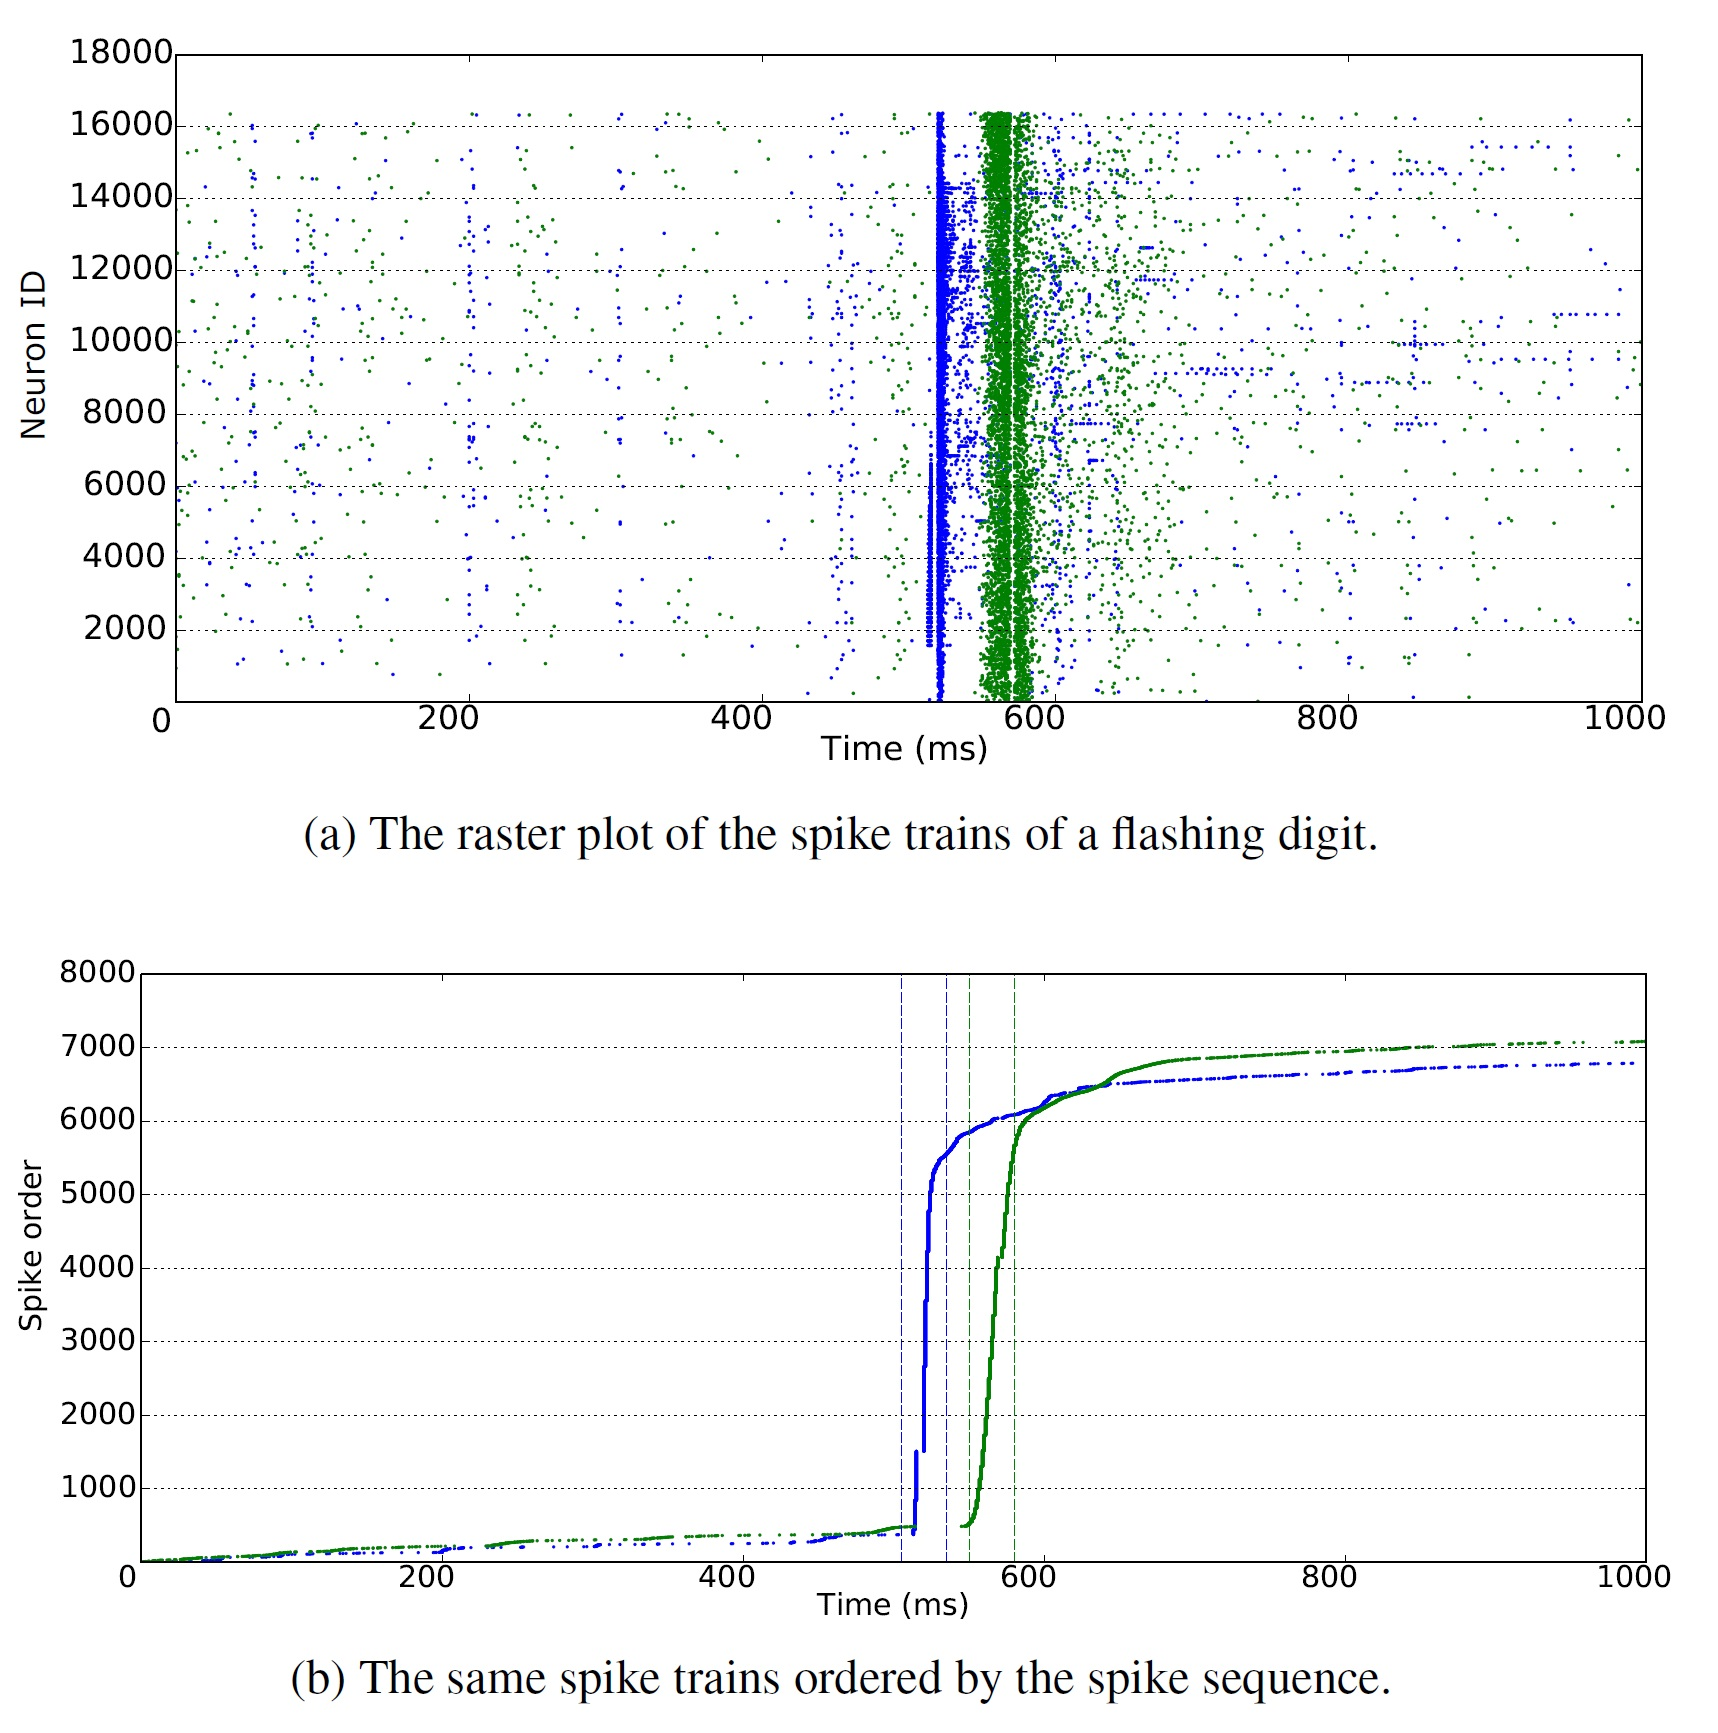
\includegraphics[width=0.8\textwidth]{pics_bench/fig5}	
	\caption{DVS sensor with flashing input.
	Blue is used for `ON' events and green for `OFF' events.
	(a) The raster plot shows spikes generated by individual neurons over time.
	It is hard to recognise the total number of spikes due to the large number of neurons involved in the figure.
	Thus all the spikes are ordered in time, and displayed in the figure below.
	(b) The raster plot shows ordered spike sequence over time.
	The total number of spikes are around $7,000$ for both `ON' and `OFF' events.
	The bursty nature of the resulting spikes is illustrated, where most of the spikes occur in a 30~ms time slot.}
	\label{fig:flash}
\end{figure}

\subsubsection{DVS Sensor Output with Moving Input}

The subset with DVS recorded moving digits is presented to address the challenges of position- and scale- invariance in computer vision.

MNIST digits were scaled to three different sizes, using smooth interpolation algorithms to increase their size from the original 28x28 pixels, and displayed on the monitor with slow motion. 
The same DVS~\cite{serrano2013128} used in Section~\ref{subsec_flash} captured the movements of the digits and generated spike trains for each pixel in its 128$\times$128 resolution.
A total of $30,000$ recordings were made: 10 digits, at 3 different scales, $1,000$ different handwritten samples for each.

\subsection{Performance Evaluation}
\label{sec:eval}
As a result of the spike-based processing used in SNN models, new concerns (outlined below) arise over performance assessment.
Therefore we propose corresponding evaluation metrics and suggest a sufficient description of SNN models in this section.
Once a model is implemented on a neuromorphic platform, the hardware performance can be evaluated by running the particular model.
This model-specific assessment provides more robust comparisons between hardware platforms thanks to using the same network topology, neuron and synaptic models, and learning rules. 
A complementary evaluation methodology is essential to provide common metrics and assess both the model-level and hardware-level performance.


\subsubsection{Model-Level Evaluation}
\label{subsec:model}

A suggested description of an SNN model is shown in Table~\ref{tb:model_eval} where the performance evaluation metrics are in bold and the SNN specific description is in italics.

Because SNNs introduce the time dimension and spike-based processing, additional performance metrics become relevant in addition to classification accuracy: these are recognition latency and the number of synaptic events.
%Both of the metrics are proposed according to the biological aspects.
Recognition latency measures how fast spikes are conveyed through the layers of network to trigger the recognition neurons.
\cite{dicarlo2012does} considers the rapid ($<$200~ms) and accurate vision recognition in the brain as the essential problem of object recognition.
For real-time systems with live visual inputs, such as robotic systems, a short response latency helps make fast decisions and take rapid action.
The latency is measured as the time difference between the first spike generated by the output layer and the first spike from the input layer.
A small total number of synaptic events generated by a recognition task indicates the efficiency of the SNN model.
A spike event is a synaptic operation evoked when one action potential is transmitted through one synapse~\cite{sharp2012power}.
Fewer spike events implies lower overall neural activity and lower energy consumption.
The number of synaptic events can be measured as ``Sopbs'', synaptic operations per biological second.
\begin{table*}[hbt!]
	\caption{SNN descriptions at the model level}
	\begin{center}
		\bgroup
		\def\arraystretch{1.5}
		\begin{tabular}{ l l l l }
			\begin{mycell}{3.7cm}Input\end{mycell} & 
			\begin{mycell}{2.5cm} Network\end{mycell} & 
			\begin{mycell}{3.5cm} Training \end{mycell} & 
			\begin{mycell}{5cm} Recognition \end{mycell} \\
			\hline
			
			\begin{leftcell}{3.7cm} - \textit{converting methods}\\- preprocessing \end{leftcell} & % preprocessing
			\begin{leftcell}{2.5cm} - topology\\- \textit{neuron and synaptic type} \end{leftcell}&  % network
			\begin{leftcell}{4cm} - supervised or not\\- \textit{learning rule} \\ - \textit{biological training time}\end{leftcell}&  % training
			\begin{leftcell}{5cm} - \textbf{classification accuracy}\\ - \textbf{\textit{response latency}}\\ - \textbf{\textit{number of synaptic events}} \\ - \textit{biological testing time}\\ - \textit{input spiking rate}  \end{leftcell}% recognition
		\end{tabular}
		\egroup
	\end{center}
	\label{tb:model_eval}
\end{table*}

Alongside the SNN evaluation metrics, a sufficient description of a network model is required so that other researchers can reproduce it and compare it with other models.
First of all, the input of an SNN model is specified.
The description includes the transformation method for converting raw images to spike trains, and the preprocessing either to images or spikes.
Filtering the raw image may ease the classification/recognition task while adding noise may require more robustness in the model.
Secondly, as with the evaluation of conventional artificial neural networks, a description of the network characteristics provides the basis for the overall performance evaluation.
Sharing the designs not only makes the model reproducible but also inspires fellow scientists to bring new points of view to the problem, generating a positive feedback loop where everybody wins.
The main characteristics include the topology and the neural and synaptic models.
The network topology defines the number of neurons used for each layer and the connections between layers and neurons.
It is essential to state the types of neural and synaptic model (e.g. current-based LIF neuron) utilised in the network and the parameters configuring them, because neural activities differ greatly between configurations.
Any non-neural classifier, sometimes added to aid the design enhance the output of the network, must also be specified.
Thirdly, the training procedure determines the recognition capability of a network model.
%A clear distinction should be made between supervised, semi-supervised and unsupervised learning.
Specifying the learning algorithm with its mechanism (supervised, semi-supervised and unsupervised) helps the reader undersdand the core features of the model.
A detailed description of new spike-based learning rules will be a great contribution to the field due to the present lack of spatio-temporal learning algorithms.
Most publications reflect the use of adaptations to existing learning rules; details on these modifications should be clear and unambiguous.
In conventional computer vision, the number of iterations of training images presented to the network play an important role.
Similarly, the biological training time determines the amount of information provided for training an SNN.
Finally in the testing phase, as well as the performance evaluation metrics stated above, specific configurations of the input spikes are also essential.
This includes details of the way samples were presented: spiking rates, and biological time per test sample.
The combination of these two factors determines how much information is presented to the network.
%Some work on SNN-based classifications of MNIST is listed in Table~\ref{tb:software_comparison}.
Following to the formatted evaluation as in Table~\ref{tb:model_eval}, Table~\ref{tb:software_comparison} lists a few SNN models of MNIST classification, although some detailed description is missing. 
%Most of these reports did not provide sufficiently detailed descriptions of the networks and the models were not completely evaluated in the way that we propose.
\begin{table*}[hbt!]
	\caption{Model-level comparison}
	\begin{center}
		\bgroup
		\def\arraystretch{1.5}
		\begin{tabular}{ l c c c c }
			$ $ &
			\begin{mycell}{1.9cm} Input\end{mycell} & 
			\begin{mycell}{3.5cm} Network\end{mycell} & 
			\begin{mycell}{3.5cm} Training \end{mycell} & 
			\begin{mycell}{3.5cm} Recognition \end{mycell} \\
			\hline
			
			%
			\begin{mycell}{2.5cm}~\cite{brader2007learning} \end{mycell} & 
			\begin{mycell}{1.9cm} Normalisation \end{mycell} & % preprocessing
			\begin{mycell}{3.5cm} Two layer, LIF neurons\end{mycell}&  % network
			\begin{mycell}{3.5cm} Semi-supervised, STDP, calcium LTP/LTD\end{mycell}&  % training
			\begin{mycell}{3.5cm} 96.5\% \end{mycell} \\% recognition
			
			%
			\begin{mycell}{2.5cm}~\cite{beyeler2013categorization} \end{mycell} & 
			\begin{mycell}{1.9cm} Scaling, V1 (edge),\\ Poisson\end{mycell} & % preprocessing
			\begin{mycell}{3.5cm} V2 (orientation),\\ and competitive decision, Izhikevich neurons\end{mycell}&  % network
			\begin{mycell}{3.5cm} Semi-supervised, STDP, \\ calcium LTP/LTD \end{mycell} &  % training
			\begin{mycell}{3.5cm} 91.6\% \\ 300~ms per test \end{mycell} \\% recognition
			
			%
			\begin{mycell}{2.5cm}~\cite{neftci2013event} \end{mycell} & 
			\begin{mycell}{1.9cm} Thresholding,\\ Synaptic current\end{mycell} & % preprocessing
			\begin{mycell}{3.5cm} Two layer RBM, \\ LIF neurons \end{mycell}&  % network
			\begin{mycell}{3.5cm} Event-driven contrastive divergence, supervised \end{mycell}&  % training
			\begin{mycell}{3.5cm} 91.9\% \\ 1~s per test\end{mycell} \\% recognition
			
			%
			\begin{mycell}{2.5cm}~\cite{diehl2015unsupervised} \end{mycell} & 
			\centering Poisson &
			\begin{mycell}{3.5cm} Two layers, LIF neurons, inhibitory feedback  \end{mycell}& 
			\begin{mycell}{3.5cm} Unsupervised, exp. STDP, %adaptive membrane potential, 
				$3,000,000$~s of training\\ $200,000$~s per iteration\end{mycell} & 
			\begin{mycell}{3.5cm} 95\% \end{mycell}\\
			
			%
			\begin{mycell}{2.5cm}~\cite{Diehl2015fast}\end{mycell}  & 
			\begin{mycell}{1.9cm} Poisson \end{mycell} & % preprocessing
			\begin{mycell}{3.5cm} ConvNet or \\Fully connected,\\ LIF neurons \end{mycell}& % network
			\begin{mycell}{3.5cm} Off-line trained with ReLU, weight normalisation \end{mycell}&   % training
			\begin{mycell}{3.5cm} 99.1\% (ConvNet), \\ 98.6\% (Fully connected);\\0.5~s per test\end{mycell}\\ % recognition    
			%
			\begin{mycell}{2.5cm}~\cite{zhao2014feedforward}\end{mycell}  & 
			\begin{mycell}{1.9cm} Thresholding \\ or DVS \end{mycell}& % preprocessing 
			\begin{mycell}{3.5cm} Simple (Gabor), \\Complex (MAX) \\and Tempotron  \end{mycell}& % network
			\begin{mycell}{3.5cm} Tempotron, supervised \end{mycell}& % training
			\begin{mycell}{3.5cm} Thresholding \\ 91.3\%, 11~s per test \\ DVS \\ 88.1\%, 2~s per test\end{mycell}\\ % recognition
			
			%
			\begin{mycell}{2.5cm} % %\cite{Stromatias2015scalable} \\ 
				This paper \end{mycell} & 
			\begin{mycell}{1.9cm} Poisson \end{mycell} & % preprocessing
			\begin{mycell}{3.5cm} Four layer RBM, \\ LIF neurons \end{mycell}&  % network
			\begin{mycell}{3.5cm} Off-line trained, unsupervised \end{mycell}&  % training
			\begin{mycell}{3.5cm} 94.94\%\\16 ms latency \\ 1.44M Sopbs\end{mycell} \\% recognition
			%
			\begin{mycell}{2.5cm} This paper \end{mycell}  & 
			\begin{mycell}{1.9cm} Poisson \end{mycell}& % preprocessing 
			\begin{mycell}{3.5cm} Fully connected decision layer, \\ LIF neurons \end{mycell}& % network
			\begin{mycell}{3.5cm} K-means clusters,\\Supervised STDP\\$18,000$~s of training \end{mycell}& % training
			\begin{mycell}{3.5cm} 92.99\%\\1~s per test\\200~ms silence \\13.82~ms latency\\$4.17$M Sopbs\end{mycell}\\ % recognition
		\end{tabular}
		\egroup
	\end{center}
	\label{tb:software_comparison}
\end{table*}

\subsubsection{Hardware-Level Evaluation}
\label{subsec:hw}

  \begin{table*}[thb!]
  	\caption{Hardware-level comparison}
  	\begin{center}
      \begin{minipage}{\textwidth}
        
        \begin{savenotes}
  		\bgroup
  		\def\arraystretch{1.4}
  		\begin{tabular}{l c c c c c c}
  			$ $ & 
  			\begin{mycell}{2.0cm} System \end{mycell} & 
  			%       \begin{minipage}{1.3cm}\centering Simulation type \end{minipage} & 
  			
  			\begin{mycell}{2.0cm} Neuron Model \end{mycell} & 
  			\begin{mycell}{2.0cm}Synaptic\\Plasticity\end{mycell} &
  			%       \begin{minipage}{1cm}\centering Axonal delays \end{minipage} & 
  			%       \begin{minipage}{1cm}\centering Synaptic model \end{minipage} & 
  			\begin{mycell}{2.0cm} Precision \end{mycell} &  
  			%       \begin{minipage}{1.2cm}\centering Synaptic precision \end{minipage} & 
  			%       \begin{minipage}{1.2cm}\centering Energy per SE \end{minipage} & 
  			%       \begin{minipage}{1.4cm}\centering Synaptic ops per Watt \end{minipage} & 
  			\begin{mycell}{2.0cm} Simulation\\Time \end{mycell} & 
  			\begin{mycell}{2.0cm} Energy \\Usage \end{mycell} 
  			%       \begin{minipage}{1.7cm}\centering Programming front-end \end{minipage}  
  			\\
  			\hline
  			% contents!
  			
  			\begin{mycell}{1.8cm} SpiNNaker \cite{stromatias2013power} \end{mycell} &
  			\begin{mycell}{2.0cm} Digital, \\Scalable \end{mycell} & 
  			\begin{mycell}{2.1cm}Programmable\\Neuron and Synapse,\\Axonal delay \end{mycell}& 
  			\begin{mycell}{2.1cm}Programmable\\learning rule\end{mycell}& 
  			\begin{mycell}{2.0cm}11- to 14-bit synapses\end{mycell} & 
  			\begin{mycell}{2.0cm} Real-time \\ Flexible time resolution \end{mycell}  &
  			\begin{mycell}{2.5cm} 8~nJ/SE \end{mycell} \\
  			%
  			\begin{mycell}{1.8cm} TrueNorth \cite{merolla2014million}\end{mycell} & \begin{mycell}{2.0cm}Digital, \\Scalable \end{mycell}& 
  			\begin{mycell}{2.0cm}Fixed models,\\Config params,\\Axonal delay\end{mycell}& 
  			\begin{mycell}{2.0cm}No plasticity\end{mycell}& 
  			\begin{mycell}{2.2cm}122 bits \\params \& states,
  				%       	 per neuron
  				\\4-bit/\\4 values\\synapse 
  				%\\(4 signed int + on/off state)
          \footnote[1]{We consider them 4-bit synapses because it is only possible to choose between 4 different signed integers and whether the synapse is active or not.}
  			\end{mycell}& 
  			\begin{mycell}{2.0cm}Real-time\end{mycell}& 
  			\begin{mycell}{2.0cm}26 pJ/SE\end{mycell} \\
  			
  			%
  			\begin{mycell}{1.8cm} Neurogrid \cite{benjamin2014neurogrid}\end{mycell} &
  			\begin{mycell}{2.0cm}Mixed-mode,\\Scalable\end{mycell} & 
  			\begin{mycell}{2.0cm}Fixed models,\\Config params\end{mycell} & 
  			\begin{mycell}{2.0cm}Fixed rule\end{mycell} & 
  			\begin{mycell}{2.0cm}13-bit shared \\ synapses\end{mycell} &
  			\begin{mycell}{2.0cm}Real-time\end{mycell} &
  			\begin{mycell}{2.0cm}941 pJ/SE\end{mycell} \\
  			%
  			\begin{mycell}{1.8cm} HI-CANN \cite{schemmel2010wafer}  \end{mycell} & \begin{mycell}{2.0cm}Mixed-mode,\\Scalable\end{mycell} &
  			\begin{mycell}{2.0cm}Fixed models,\\Config params\end{mycell}& 
  			\begin{mycell}{2.0cm}Fixed rule\end{mycell}& 
  			\begin{mycell}{2.0cm}4-bit/\\16 values\\synapses\end{mycell}& 
  			\begin{mycell}{2.0cm}Faster than\\ real-time
                             \footnote[2]{A maximum speed-up of up to $10^5$ times real time has been reported.}
        \end{mycell}&
  			\begin{mycell}{2.0cm} 7.41 nJ/SE\\(network only) \end{mycell}\\
  			%
  			\begin{mycell}{1.8cm} HiAER-IFAT \cite{yu201265k}\end{mycell} & 
  			\begin{mycell}{2.0cm}Mixed-mode,\\Scalable\end{mycell} &
  			\begin{mycell}{2.0cm}Fixed models,\\Config params\end{mycell}& 
  			\begin{mycell}{2.0cm}No plasticity\end{mycell} &  
  			\begin{mycell}{2.0cm}Analogue neuron/synapse\end{mycell} & 
  			Real-time&
  			\begin{mycell}{2.0cm}22-pJ/SE\\\cite{park201465k}\end{mycell}
  			
  			%dummy update text
  		\end{tabular}
  		\egroup

\end{savenotes}
\end{minipage}
  	\end{center}
  	\label{tb:hardware_comparison}
  \end{table*}


Neuromorphic systems can be categorised as analogue, digital, or mixed-mode analogue/digital, depending on how neurons, synapses and spike transmission are implemented. %VLSI circuits. 
Some analogue implementations exploit sub-threshold transistor dynamics to emulate neurons and synapses directly in hardware~\cite{indiveri2011neuromorphic} and are more energy-efficient while requiring less area than their digital counterparts~\cite{joubert2012hardware}. However, the behaviour of analogue circuits is hard to control through the fabrication process due to transistor mismatch~\cite{indiveri2011neuromorphic,pedram2006thermal,linares2003compact}, and achievable wiring densities render direct point-to-point connections impractical for large-scale systems. The majority of mixed-mode analogue/digital neuromorphic platforms, such as the High Input Count Analog Neural Network (HI-CANN)~\cite{schemmel2010wafer}, Neurogrid~\cite{benjamin2014neurogrid}, HiAER-IFAT~\cite{yu201265k}, use analogue circuits to emulate neurons and digital packet-based technology to communicate spikes as AER events. This enables reconfigurable connectivity patterns, while spike timing is expressed implicitly since typically a spike reaches its destination in less than a millisecond, thus fulfilling the real-time requirement. Digital neuromorphic platforms such as TrueNorth~\cite{merolla2014million} use digital circuits with finite precision to simulate neurons in an event-driven manner to minimise the active power dissipation. Such systems suffer from limited model flexibility, since neurons and synapses are fabricated directly in hardware with only a small subset of parameters under the control of the researcher. 
The SpiNNaker many-core neuromorphic architecture~\cite{furber2014spinnaker} uses low-power programmable cores and scalable event-driven communications hardware allowing neural and synaptic models to be implemented in software.
While software modelling provides great flexibility, digital platforms generally have reduced precision (due to the inherent discretisation) and higher energy consumption when compared to analogue platforms. Furthermore, the processing cores used in SpiNNaker chips perform better when using integer or fixed-point arithmetic~\cite{Hopkins2015Accuracy}.
And the requirement for the models to run in real time leads to constraints a the complexity of model that can be supported.

A direct comparison between neuromorphic platforms is a non-trivial task due to the different hardware implementation technologies as mentioned above.
%Qian Liu modified
Table~\ref{tb:hardware_comparison} attempts to describe the neuromorphic hardware platforms with reference to different aspects of SNN simulation.
The scalability of a hardware platform determines the network size limit of a neural application running on it.
Considering the various neural and synaptic models, plasticity learning rules and lengths of axonal delays, a programmable platform offers flexibility to support diverse SNNs while a hard-wired system supporting only specific models wins for its energy-efficiency and simpler design and implementation.
The classification accuracy of an SNN running on a hardware system can be different from the software simulation, since hardware implementations may impose limits on the precision used for the membrane potential of neurons (for the digital platforms) and the synaptic weights.
%Thus comparison metrics is supposed to include precision as a major assessment of the system performance.
Simulation time is another important measure when running large-scale networks on hardware.
Real-time implementation is an essential requirement for robotic systems because of the real-time input from the neuromorphic sensors.
Running faster than real time is attractive for large and long simulations.
%Finer time resolution plays an important role in precision-sensitive neural models or in sub-millisecond tasks~\cite{lagorce2015breaking}.
%Qian Liu done
It is interesting to comparing the performance of each platform in terms of energy requirements, especially if the platform targets mobile applications and robotics.
Some researchers have suggested the use of energy per synaptic event (J/SE)~\cite{sharp2012power,stromatias2013power} as an energy metric because the large fan in and out of a neuron means that synaptic processing tends to dominate the total energy dissipation during a simulation.
\cite{merolla2014million} proposed the number of synaptic operations per second per Watt (Sops/W).
These two measures are equivalent, since J/SE$\times$Sops/W = 1.
To investigate the power usage in detail, \cite{Diamond2016comparing} included the power drawn by the attached workstations.
This work indicated the power variation by each task over time.

%Qian Liu modified
However, the typical reported simulation time and energy use for the various platforms is under different SNN models, making the comparisons problematic.
Model-specific hardware metrics would provide robust comparisons between platforms and expose how different networks influence the metrics on particular hardware.
The proposed evaluation metrics (see Table~\ref{tb:hw_eval}) consist of the feasibility, classification accuracy, simulation time and energy use.
A particular SNN model is feasible to run on a particular hardware platform only when the network size is under the platform's limit, the neural and synaptic models are supported, and the learning rule is implemented.
CA also plays a role in hardware evaluation because of the precision limits that may be imposed by the platform.
Due to the limited hardware resources, simulation time may, likewise, accelerate or slow down according to the network topology and spike dynamics.
Similarly, energy costs vary with different networks and neural and synaptic models.
%The system performance will be assessed on the accuracy, simulation time and energy use running the network. 
%Table~\ref{tb:hardware_comparison} aims to summarise the aforementioned hardware comparison metrics.
\begin{table*}[hbt!]
	\caption{Hardware level evaluation of model specific SNN simulation}
	\begin{center}
		\bgroup
		\def\arraystretch{1.5}
		\begin{tabular}{ l l l l }
			\begin{mycell}{5cm} Hardware Description \end{mycell} & 
			\begin{mycell}{5cm} Evaluation Metrics \end{mycell} \\
			\hline
			\begin{leftcell}{5cm} - Digital/Analogue \\- Scalability\\- Neuron models supported\\- Synapse models supported\\- Synaptic plasticity \\- Precision \end{leftcell}&  % training
			\begin{leftcell}{5cm} - feasibility\\- classification accuracy \\- simulation time \\- energy use \end{leftcell}% recognition
		\end{tabular}
		\egroup
	\end{center}
	\label{tb:hw_eval}
\end{table*}

\section{Results}
\section{Summary}
This paper puts forward the NE dataset as a baseline for comparisons of vision based SNN models and neuromorphic platforms.
It contains spike-based versions of existing widely-used databases in the vision recognition field.
Since new problems will continue to arise before vision becomes a solved question, the dataset will evolve as research progresses. 
The conversion methods for transforming images and videos into spike trains will advance. The number of vision datasets will increase and the corresponding evaluation methodologies will evolve.
The dataset aims to provide unified spike-based vision benchmarks and complementary evaluation methodologies to assess the performance of SNN algorithms.

The first version of the dataset is published as NE15-MNIST, which contains four different spike representations of the MNIST stationary hand-written digit database.
The Poissonian subset is intended for benchmarking existing rate-based recognition methods.
The rank-order-encoded subset, FoCal, encourages research into spatio-temporal algorithms on recognition applications using only small numbers of input spikes.
Fast recognition can be verified on the DVS recorded flashing input subset, since just 30~ms of useful spike trains are recorded for each image.
Looking forward, the continuous spike trains captured from the DVS recorded moving input can be used to test mobile neuromorphic robots.
\cite{orchard2015convert} have presented a neuromorphic dataset using a similar approach, but the spike trains were obtained with micro-saccades.
This dataset aims to convert static images to neuromorphic vision input, while the recordings of moving input in this paper are intended to promote position-invariant recognition.
Therefore, the datasets complement each other..

The complementary evaluation methodology is essential to assess both the model-level and hardware-level performance of SNNs.
In addition to classification accuracy, response latency and the number of synaptic events are specific evaluation metrics for spike-based processing.
Moreover, it is important to describe an SNN model in sufficient detail to share the network design, and relevant SNN characteristics were highlighted in the paper.  
%For a neural network model, its topology, neuron and synapse models, and training methods are major descriptions for any kind of neural networks, including SNNs.
%While the recognition accuracy, network latency and also the biological time taken for both training and testing are specific performance measurements of a spike-based model.
The network size of an SNN model that can be built on a hardware platform will be constrained by the scalability of the hardware.
Neural and synaptic models are limited to the ones that are physically implemented, unless the hardware platform supports programmability.
Any attempt to implement an on-line learning algorithm on neuromorphic hardware must be backed by synaptic plasticity support.
Therefore running an identical SNN model on different neuromorphic hardware exposes the capabilities of such platforms.
If the model runs smoothly on a hardware platform, it then can be used to benchmark the performance of the hardware simulator in terms of simulation time and energy usage.
Classification accuracy (CA) is also a useful metric for hardware evaluation because of the limited precision of the membrane potential and synaptic weights.

Although spike-based algorithms have not surpassed their non-spiking counterparts in terms of recognition accuracy, they have shown great performance in response time and energy efficiency.
This dataset makes the comparison of SNNs with conventional recognition methods possible by using converted spike representations of the same vision databases.
As far as we know, this is the first attempt at benchmarking neuromorphic vision recognition by providing public a spike-based dataset and evaluation metrics.
In accordance with the suggestions from~\cite{tan2015bench}, the evaluation metrics highlight the strengths of spike-based vision tasks and the dataset design also promotes the research into rapid and low energy recognition (e.g. flashing digits).
Two benchmark systems were evaluated using the Poissonian subset of the NE15-MNIST dataset.
%The models were described and their performance on accuracy, network latency, simulation time and energy usage were presented.
These example benchmarking systems demonstrated a recommended way of using the dataset, describing the SNN models and evaluating the system performance.
%They provide a baseline for comparisons and encourage improved algorithms and models to make use of the dataset.
The case studies provide baselines for robust comparisons between SNN models and their hardware implementations.
%As the dataset grows, it will allow new problems to be investigated by researchers, which should allow the identification of future directions and, in consequence, advance the field.

%\subsection{The future direction of a developing database}
\subsection{The future direction of an evolving database}
The database will be expanded by converting more popular vision datasets to spike representations.
As mentioned in Section~\ref{sec:intro}, face recognition has become a hot topic in SNN approaches, however there is no unified spike-based dataset to benchmark these networks.
Thus, the next development step for our dataset is to include face recognition databases.
While viewing an image, saccades direct high-acuity visual analysis to a particular object or a region of interest and useful information is gathered during the fixation of several saccades in a second.
It is possible to measure the scan path or trajectory of the eyeball and those trajectories show particular interest in eyes, nose and mouth while viewing a human face~\cite{yarbus1967eye}.
Therefore, our plan is also to embed modulated trajectory information to direct the recording using DVS sensors to simulate human saccades.

There will be more methods and algorithms for converting images to spikes.
Although Poisson spikes are the most commonly used external input to an SNN system, there are several \textit{in-vivo} recordings in different cortical areas showing that the inter-spike intervals (ISI) are not Poissonian~\cite{deger2012statistical}. 
Thus~\cite{deger2012statistical} proposed new algorithms to generate superposition spike trains of Poisson processes with dead-time (PPD) and of Gamma processes.
Including novel spike generation algorithms in the dataset is one aspect of future work which will be carried out.

%While the major stumbling crux of the computer object recognition systems lies in the invariance problem.
Each encounter of an object on the retina is unique, because of the illumination (lighting condition), position (projection location on the retina), scale (distance and size), pose (viewing angle), and clutter (visual context) variabilities.
But the brain recognises a huge number of objects rapidly and effortlessly even in cluttered and natural scenes.
In order to explore invariant object recognition, the dataset will include the NORB (NYU Object Recognition Benchmark) dataset~\cite{lecun2004learning}, which contains images of objects that are first photographed in ideal conditions and then moved and placed in front of natural scene images.

Action recognition will be the first problem of video processing to be introduced in the dataset.
The initial plan is to use the DVS retina to convert the KTH and Weizmann benchmarks to spiking versions.
Meanwhile, providing a software DVS retina simulator to transform frames into spike trains is also on the schedule.
By doing this, a huge number of videos, such as those in YouTube, can automatically be converted into spikes, therefore providing researchers with more time to work on their own applications.

In all, it is impossible for the dataset proposers to provide enough datasets, converting methods and benchmarking results, thus we encourage other researchers to contribute to the dataset.
Researchers can contribute their data to the dataset, allowing future comparisons using the same data source;
they can share their spike conversion algorithms by generating datasets to promote the corresponding recognition methods;
and neuromorphic hardware owners are welcome to provide benchmarking results to compare their system's performance.